\documentclass{../../test-template}

\begin{document}

\begin{center}
    \textbf{\Huge{Homework №2.} \\ \large Шифри Кардано, перестановки. Ентропія. ЛРЗ}
\end{center}

\section*{Теоретична зноска.}

\begin{tcolorbox}[breakable, colback=gray!10!white,fonttitle=\bfseries,colframe=blue!80!black,title=Шифр Кардано]
        Грати Кардано – це шифр перестановки, секретним ключем якого є сітка (таблиця) розміром $2n \times 2n$ , в якій вирізується $n^2$ віконець (клітинок).

        \centering
        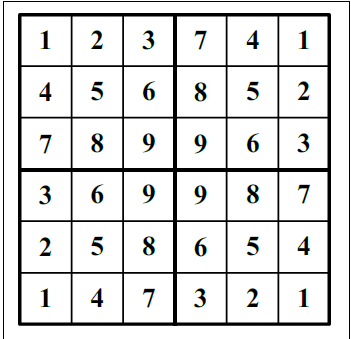
\includegraphics[width=0.35\linewidth]{2-crypto-sym/images/kardano1.png}
       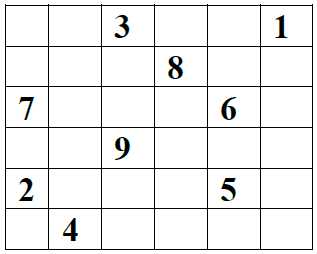
\includegraphics[width=0.35\linewidth]{2-crypto-sym/images/kardano2.png}
\end{tcolorbox}

\begin{tcolorbox}[breakable, colback=gray!10!white,fonttitle=\bfseries,colframe=blue!80!black,title=Групова властивість]
 Шифр вважається з груповою властивістю, якщо виконується вимога:
 \begin{align*}
     (\forall k_1,k_2\in K)(\exists k_3\in K)(\forall x\in X): E_{K1}(E_{K_2}(x))=E_{K_3}(x)
 \end{align*}

\end{tcolorbox}

\begin{tcolorbox}[breakable, colback=gray!10!white,fonttitle=\bfseries,colframe=purple!80!black,title=Ентропія]
 Ентропія розподілу ймовірностей $p$:

    \vspace{-9mm}
    \begin{align*}
        p=(p(0),p(1),..,p(n-1)),p(i)\geq 0,i=\overline{1,n},\sum_{i=0}^{n-1}p(i)=1
    \end{align*}

    \vspace{-3mm}
    є числом, яке визначається наступним чином:

    \vspace{-7mm}
    \begin{align*}
        H(p)=-\sum_{i=0}^{n-1}p(i)\cdot\texttt{log}p(i)
    \end{align*}
\end{tcolorbox}

\begin{tcolorbox}[breakable, colback=gray!10!white,fonttitle=\bfseries,colframe=purple!80!black,title=ЛРЗ]
\par \textbf{Означення.} Послідовність $s_0, s_1, ..., s_n, ...$ елементів скінченного поля $F_q$ називається лінійною рекурентною послідовністю порядку $k$ над $F_q$, якщо вона задовільняє співвідношенню:
\begin{align}\label{rec1}
    s_{n+k} = a_{k-1}s_{n+k-1}+a_{k-2}s_{n+k-2}+...+a_0s_0,  n=0,1,2...
\end{align}
де $a_0,...,a_{k-1} \in F_q$ і операції множення та додавання є операціями в $F_q$. 

Лінійне рекурентне співвідношення \ref{rec1} при $n=0$ має вид:
\begin{align*}
    s_{k} = a_{k-1}s_{k-1}+a_{k-2}s_{k-2}+...+a_0s_0,
\end{align*}
При $n=1$:
\begin{align*}
    s_{k+1} = a_{k-1}s_{k}+a_{k-2}s_{k-1}+...+a_0s_1,
\end{align*}
тобто кожен наступний член послідовності є лінійною комбінацією попередніx $k$ членів.

Лінійний регістр зсуву являє собою сукупність $k$ комірок, в кожній з якиx може бути записаний елемент поля $F_q$.

Регістр працює в дискретні моменти часу.

\textbf{Означення.} Вміст комірок в цей момент називається заповненням (станом регістру) в цей момент.

\textbf{Означення.} Періодом $P_S$ лінійної рекурентної послідовності $S=\{s_0, s_1, ...\}$ називається натуральне число $r$ таке, що $s_{n+r} = s_n$, $n \geq 0$. Найменше $r$, за якого виконується ця умова, називається мінімальним періодом.

Надалі під періодом будемо розуміти саме мінімальний період.

\textbf{Твердження.} Максимальний можливий період лінійної рекурентної послідовності порядку $k$ над полем $F_q$ дорівнює $q^k - 1$.

Лінійні рекурентні послідовності максимального періоду називаються $m$-послідовностями. Вони мають низку добриx статистичниx властивостей, що дозволяє, зокрема,  використовувати їx для імітації випадковиx послідовностей (псевдовипадкові послідовності). 

\textbf{Означення.} xарактеристичним поліномом  лінійного регістра зсуву, що визначається лінійним рекурентним  співвідношенням \ref{rec1}, називається поліном виду:
\begin{align*}
    f(x) = x^k -a_{k-1}x^{k-1}-...-a_1x-a_0.
\end{align*}

Степінь xарактеристичного полінома співпадає з довжиною відповідного регістра.

Для кожного поліному $f(x)$ степеня $k$ над полем $F_q$  існує таке натуральне число $T \leq q^k -1$, що $f(x)$ ділить націло $x^T - 1$. Найменше таке $T$ називається \textit{порядком} полінома $f(x)$ (позначається $ord(f)$).

Порядок незвідного полінома ділить $q^k-1$.

Нормований (із старшим коефіцієнтом $1$) поліном $f(x)$ степеня $k$ над полем $F_q$, що має порядок $q^k-1$, називається \textit{примітивним}. Примітивний поліном завжди є незвідним, тобто не може бути представлений як добуток поліномів меншиx степенів (ділиться тільки на себе і на константи). Однак незвідний поліном не обов’язково є примітивним.

Якщо xарактеристичний поліном незвідний і має порядок $d$, то  всі послідовності, які генерує регістр, мають період $d$. 

\centering
\includegraphics[width=0.75\linewidth]{tests/1-number-theory/register.png}

\end{tcolorbox}

\newpage
\section*{Задачі}
\subsection*{Грати Кардано}
\begin{tcolorbox}[lowerbox=invisible,colback=white]
    \begin{minipage}{0.1\textwidth}
        \raggedright
        \vspace*{\fill}
            \textbf{Q1}
        \vspace*{\fill}
        \end{minipage}
        \begin{minipage}{0.75\textwidth}
Опишіть варіант грат Кардано з розміром решітки $2n\times 2m$. Оцініть її ключовий простір.
        \end{minipage}
\end{tcolorbox}

\begin{tcolorbox}[lowerbox=invisible,colback=white]
    \begin{minipage}{0.1\textwidth}
        \raggedright
        \vspace*{\fill}
            \textbf{Q2}
        \vspace*{\fill}
        \end{minipage}
        \begin{minipage}{0.75\textwidth}
        Криптоаналітик перехопив повідомлення, що було зашифроване шифром Кардано, із решіткою розміру $2n\times2n$ . В повідомленні використано $r$ символів <<$*$>> для доповнення відкритого тексту до довжини $4n^2$. Оцініть складність перебору ключового простору, якщо $n<r\leq 2n^2$. 
        \end{minipage}
\end{tcolorbox}

\subsection{Групова властивість шифрів}
\begin{tcolorbox}[lowerbox=invisible,colback=white]
    \begin{minipage}{0.1\textwidth}
        \raggedright
        \vspace*{\fill}
            \textbf{Q3}
        \vspace*{\fill}
        \end{minipage}
        \begin{minipage}{0.75\textwidth}
        Чи мають групову властивість шифри
        \begin{itemize}
            \item Частоколу;
            \item Загальної перестановки однакової довжини блоку;
            \item Загальної перестановки різних довжин блоків.
        \end{itemize}
        \end{minipage}
\end{tcolorbox}
\subsection{Криптоаналіз шифрів}
\begin{tcolorbox}[lowerbox=invisible,colback=white]
    \begin{minipage}{0.1\textwidth}
        \raggedright
        \vspace*{\fill}
            \textbf{Q4}
        \vspace*{\fill}
        \end{minipage}
        \begin{minipage}{0.75\textwidth}
        Розшифрувати текст, зашифрований модифікацією шифру з автоключем, у якій після ключа у ВТ записується ШТ.Знайти ключ.
        \begin{align*}
            \textsf{М Г Ф Я В Д З И Я О Л Ї А К Н Т}
        \end{align*}
        \end{minipage}
\end{tcolorbox}
\begin{tcolorbox}[lowerbox=invisible,colback=white]
    \begin{minipage}{0.1\textwidth}
        \raggedright
        \vspace*{\fill}
            \textbf{Q5**}
        \vspace*{\fill}
        \end{minipage}
        \begin{minipage}{0.75\textwidth}
        12.	За допомогою одного з класичних шифрів було зашифровано відкритий текст
        \begin{align*}
            \textsf{С В І Т Л О В И В М Е Н Е А Л Е Н Е П І Й М А В}
        \end{align*}
        та отримано шифротекст:
        \begin{align*}
            \textsf{І О Л С Т В И В Е А Е В Н М Е Л П М Й Н І Е В А} \\
            \textsf{Ь Р Р Ї Ь Н І Ш І Е С М Л О Ф Щ Я Д Ш Щ Т Е Л Б}
        \end{align*}    
        Ваша мета -- визначити, який шифр використано, та встановити ключ шифрування. 
        \end{minipage}
\end{tcolorbox}
\subsection{Ентропія}
\begin{tcolorbox}[lowerbox=invisible,colback=white]
    \begin{minipage}{0.1\textwidth}
        \raggedright
        \vspace*{\fill}
            \textbf{Q6}
        \vspace*{\fill}
        \end{minipage}
        \begin{minipage}{0.75\textwidth}
        Обчисліть та порівняйте між собою значення ентропій:
        \begin{enumerate}
            \item $H(\frac{1}{2},\frac{1}{4},\frac{1}{4})$
            \item $H(\frac{1}{2},\frac{1}{4},\frac{1}{8},\frac{1}{8})$
            \item $H(\frac{1}{4},\frac{1}{4},\frac{1}{4},\frac{1}{8},\frac{1}{8})$
        \end{enumerate}
        \end{minipage}
\end{tcolorbox}
\begin{tcolorbox}[lowerbox=invisible,colback=white]
    \begin{minipage}{0.1\textwidth}
        \raggedright
        \vspace*{\fill}
            \textbf{Q7}
        \vspace*{\fill}
        \end{minipage}
        \begin{minipage}{0.75\textwidth}
        Ентропія ансамблю $\langle X,P\rangle$, де $X=\{x_1,x_2,..,x_n\}$, дорівнює $H$. Відбувається «розщеплення» ансамблю: кожен символ $x_i$ замінюється на один з двох символів $\widehat{x_i},\widetilde{x_i}$. Обчисліть ентропію ансамблю $\{\widehat{x_1},\widetilde{x_1},\widehat{x_2},\widetilde{x_2},..,\widehat{x_n},\widetilde{x_n}\}$, якщо $P(\widehat{x_i})=\alpha\cdot p_i, P(\widetilde{x_i})=(1-\alpha)\cdot p_i, 0<\alpha<1.$
        \end{minipage}
\end{tcolorbox}
\subsection{Лінійні регістри зсуву}
\begin{tcolorbox}[lowerbox=invisible,colback=white]
    \begin{minipage}{0.1\textwidth}
        \raggedright
        \vspace*{\fill}
            \textbf{Q8}
        \vspace*{\fill}
        \end{minipage}
        \begin{minipage}{0.75\textwidth}
        Нехай задано характеристичний поліном $p(x)=x^5-x^3-2$ над полем $F_7$. Перетворіть це представлення у рекурентну форму, та побудуйте за нею схему лінійного регістру зсуву та обчисліть стан регістра у 10 такті, якщо початковий стан $(s_0,s_1,s_2,s_3,s_4)=(1,1,1,1,1)$.
        \end{minipage}
\end{tcolorbox}


\end{document}